While the greedy algorithm allows us to find near optimals for problems where we have perfect information about the
problem case like the job utility, this may be private information that the job owner doesnt want to reveal also
server would want to get paid for that work that they do. \\
We propose a iterative auction where the job owner doesnt have to reveal it's true utility. In normal VCG auction,
then the auctioneer will solve the problem to maximise the social welfare (total utility of allocated jobs) and must find the optimal solution.
Then for each job and server, the job or server is removed from the problem case and the optimal is solved for that as well
with the server's revenue it is paid and the job's cost being the social welfare of the optimal solution minus the
social welfare of the optimal without the job or server. This is extremely slow and unscalable because of this so is not
used often however has the properties that it is individually rational, truthful bidding and incentive compatible. \\
Our iterative auction uses the idea of VCG so that when a job asks to run on a server then the server will calculate
current revenue of the jobs running minus the revenue if the new job must be running on the server plus a price increase
factor. This is then the price for the job to run on the server as the new allocation with the job would be to a greater
revenue for the server than is currently allocated.

\subsection{Iterative Auction algorithm}\label{subsec:iterative-auction-algorithm}
\begin{lstlisting}[language=Python]
unallocated_jobs = jobs
while len(unallocated_jobs):
    # Select a job, can be at random
    job = unallocated_jobs[0]

    # Calculate the minimum job price on all of the servers
    job_price, allocation_info = min((evaluate_job_price(job, server, epsilon=epsilon)
                                     for server in servers), key=lambda bid: bid[0])
        # Check if the job can pay the minimum price
        if job_price <= job.utility:
            # Uses the allocation info to create the new allocation on the selected server
            allocate_job(job_price, job, allocation_info, unallocated_jobs)
        else:
            # Remove job as the job can be run ever at a price lower than the job's true utility
            unallocated_jobs.remove(job)
\end{lstlisting}

\section{Iterative Auction Results}\label{sec:auction-results}
\begin{figure}[H]
    \centering
    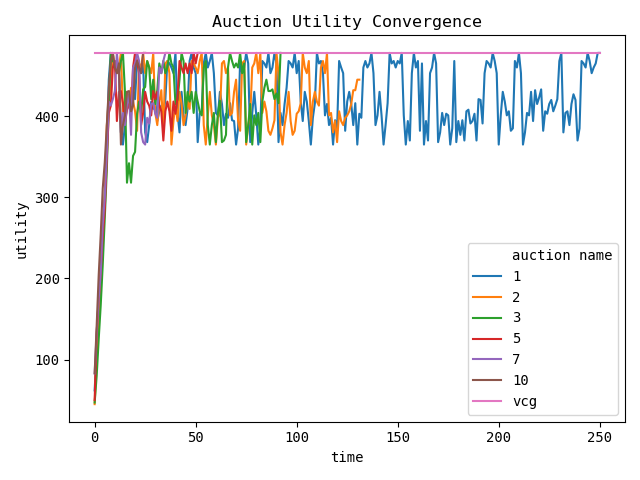
\includegraphics{../results/auction_utility_convergence.png}
    \caption{Auction Utility Convergence}
\end{figure}

%% TODO iterative auction price difference to vcg
